\documentclass[a4paper, 12pt]{mcshw}
\begin{document}
\Letsmaketitle{}
\begin{enumerate}
    \item What is the expected number of squares (4-cycles) in $G(n, \frac{d}{n})$ What is the expected number of 4-cliques in $G(n, \frac{d}{n})$?
        \begin{solution}
            Let $X$ be the number of squares and $Y$ be the number of 4-cliques. 
            \begin{align*}
                E(X) &= \frac{1}{2}\frac{n(n - 1)(n - 2)(n - 3)}{4}(\frac{d}{n})^4\\
                &= \frac{d^4(n - 1)(n - 2)(n - 3)}{8n^3}
            \end{align*}
            \begin{align*}
                E(Y) &= \frac{n(n - 1)(n - 2)(n - 3)}{4!}(\frac{d}{n})^6\\
                &= \frac{d^6(n - 1)(n - 2)(n - 3)}{24n^5}
            \end{align*}
        \end{solution}
    \item Search for \textit{WWW} for an undirected graph or a data base that can be counted to a graph. find the connected components and count the number of each size.
        \pagebreak
        \begin{solution}
            I find a dataset in \textbf{http://snap.stanford.edu/data/egonets-Facebook.html}, which provides 'circles'(or 'friends list')from Facebook.  This data was collected from survey participants using this Facebook app. For the convenience of computation, I simply remove the node with index zero, and finally get a graph which has 4038 nodes and 88233 edges.
            Here is a piece of Mathematica code to deal with it.
            \begin{center}
                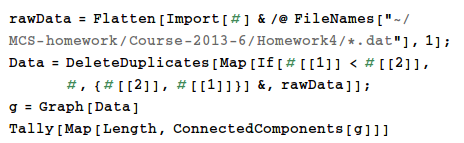
\includegraphics[height=4cm]{1.png}
            \end{center}
            And here is what the network looks like
            \begin{center}
                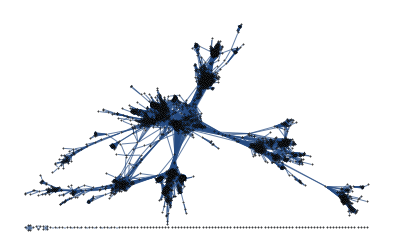
\includegraphics[height=7cm]{2.png}
            \end{center}
            And the commponents' size distribution, in the form '\{size, count\}'
            \begin{center}
                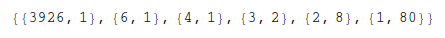
\includegraphics[height=1cm]{3.png}
            \end{center}
        \end{solution}
\end{enumerate}
\end{document}
